% DO NOT COMPILE THIS FILE DIRECTLY!
% This is included by the other .tex files.

\begin{frame}[t,plain]
\titlepage
\end{frame}

\begin{frame}[t]{The Lua Language}
\begin{itemize}
\item<1-> Our first task in training was to learn basic concepts of LUA. 
\item<2-> Lua is a powerful, fast, lightweight, embeddable scripting language.
\item<3-> It is currently the leading scripting language in games.
\end{itemize}
\end{frame}

\begin{frame}[t]{QT creator \& LibreCAD v3}
\begin{itemize}
\item<1-> First we installed Qt creater, then build and run LibreCAD v3. Then we started working with LibreCAD and made some creative design in it.
\item<2-> Qt Creator is a cross-platform C++, JavaScript and QML Integrated Development Environment (IDE) which is part of the SDK for the Qt GUI Application development framework.
\item<3-> LibreCAD is a free Computer Aided Design (CAD) application for 2D design.
\end{itemize}
\end{frame}

\watermarkoff
\begin{frame}[t,fragile]{Some Designs Using LUA in LibreCAD v3}
\begin{itemize}
\item Basic Shapes
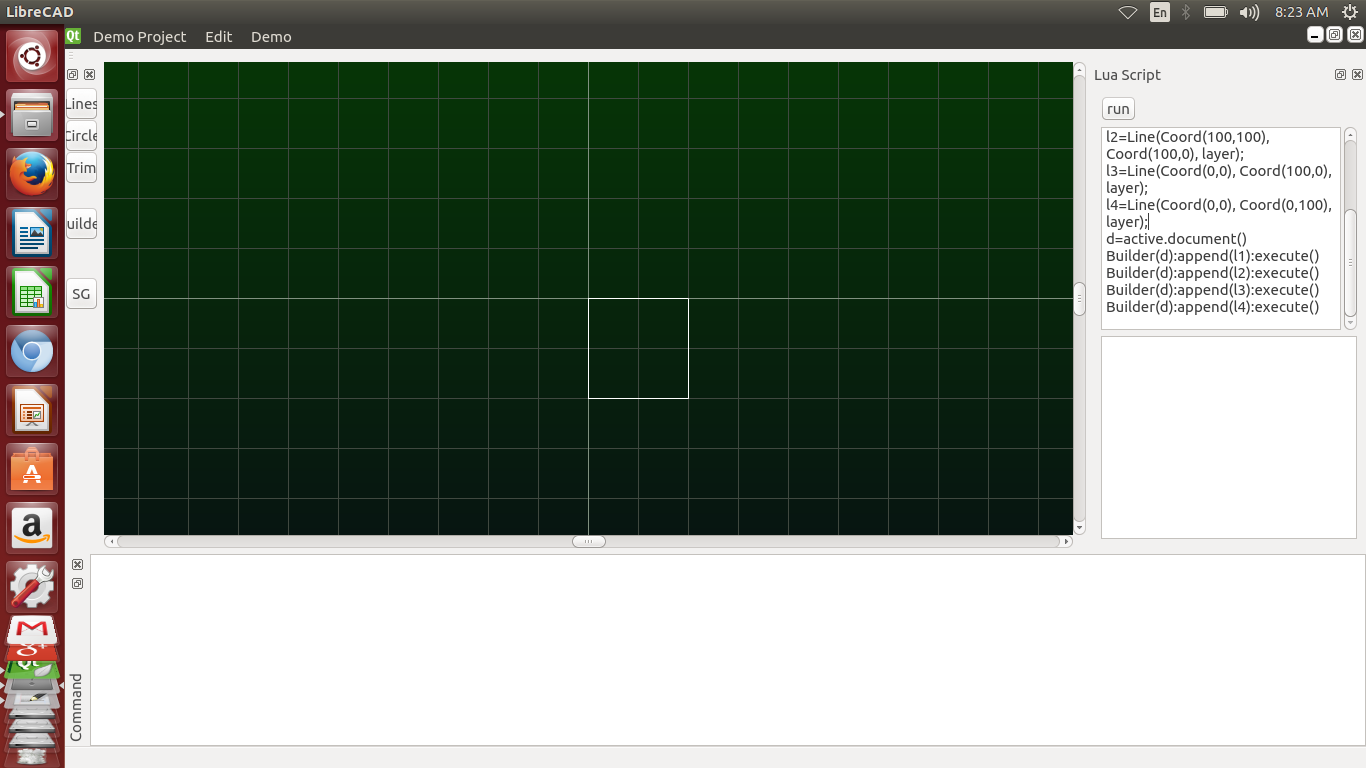
\includegraphics[scale=0.1]{square.png}
\hspace*{1\baselineskip}
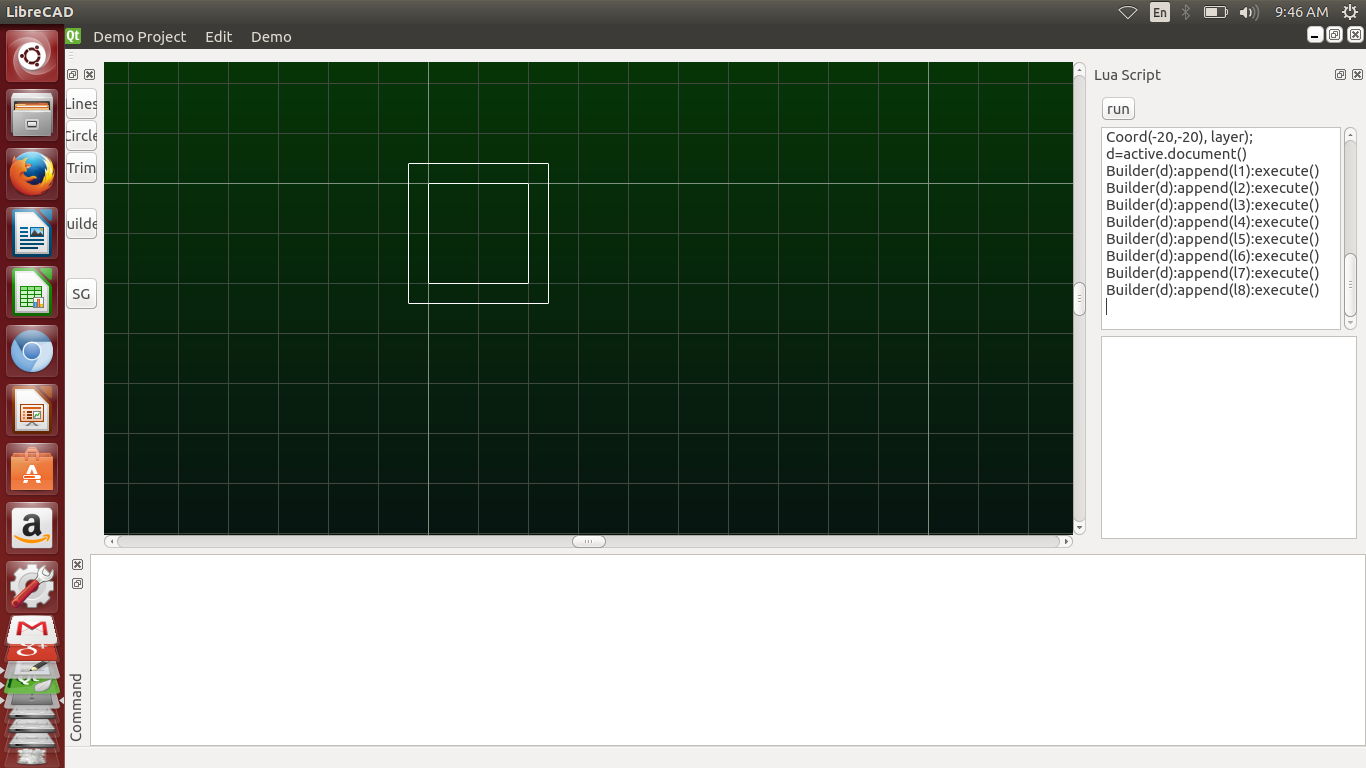
\includegraphics[scale=0.1]{dsquare.png}
\vspace*{1\baselineskip}
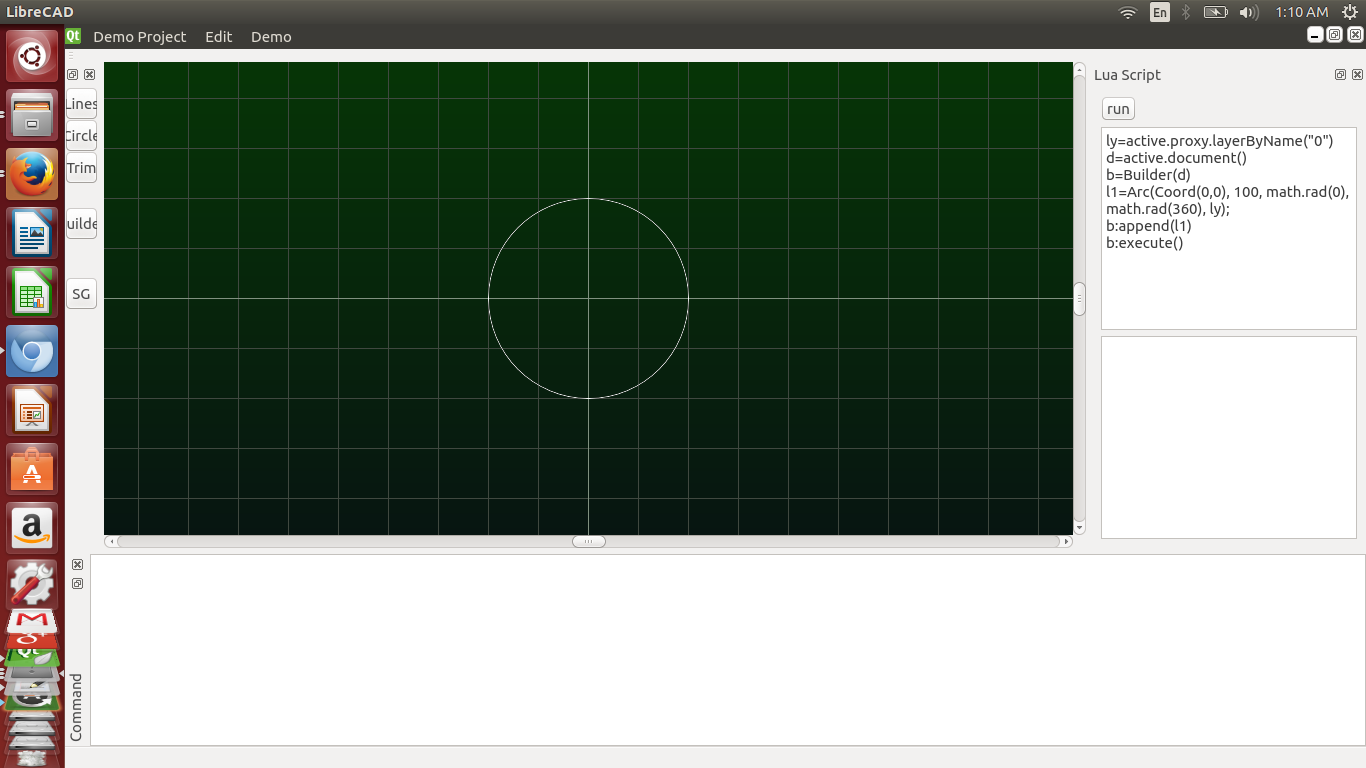
\includegraphics[scale=0.1]{circle.png}
\hspace*{1\baselineskip}
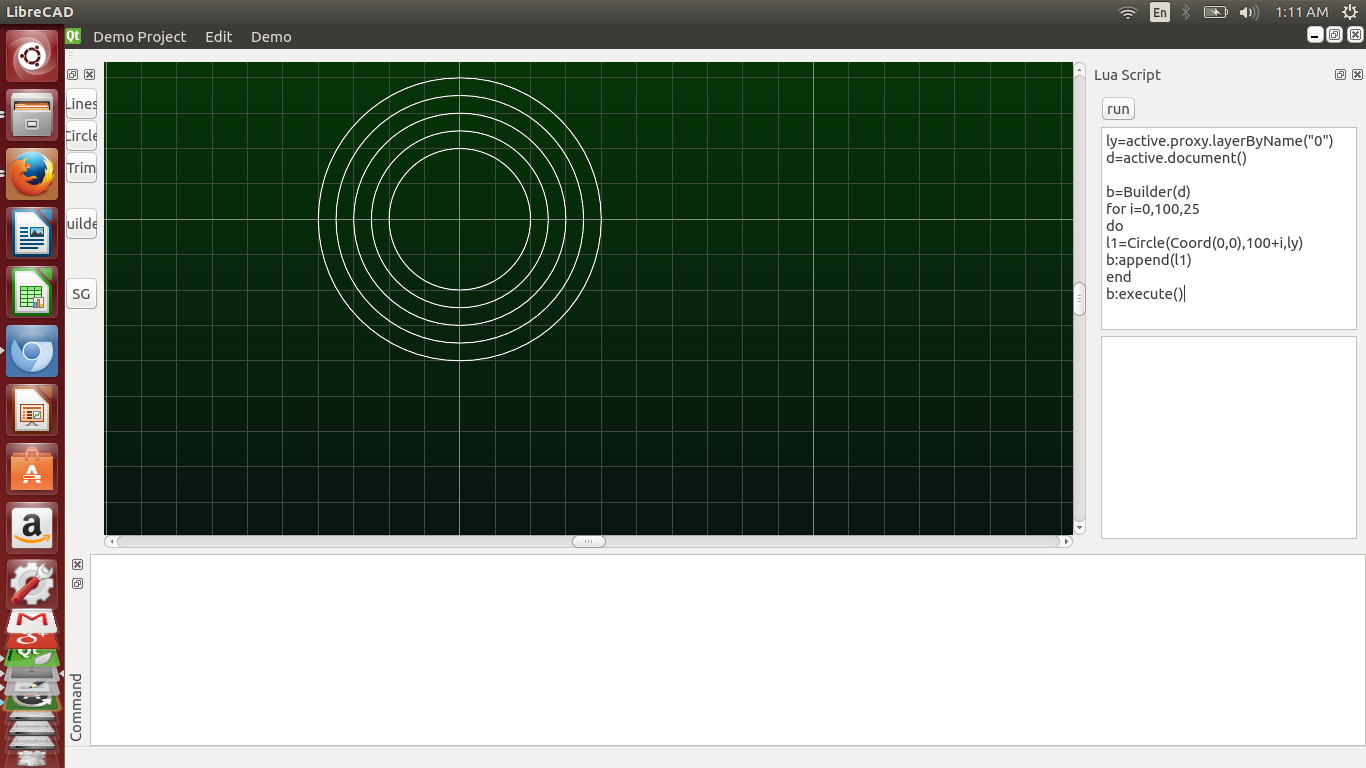
\includegraphics[scale=0.1]{concircle.png} 
\end{itemize}
\end{frame}

\begin{frame}[t,fragile]{Some Designs Using LUA in LibreCAD v3}
\begin{itemize}
\item Logos
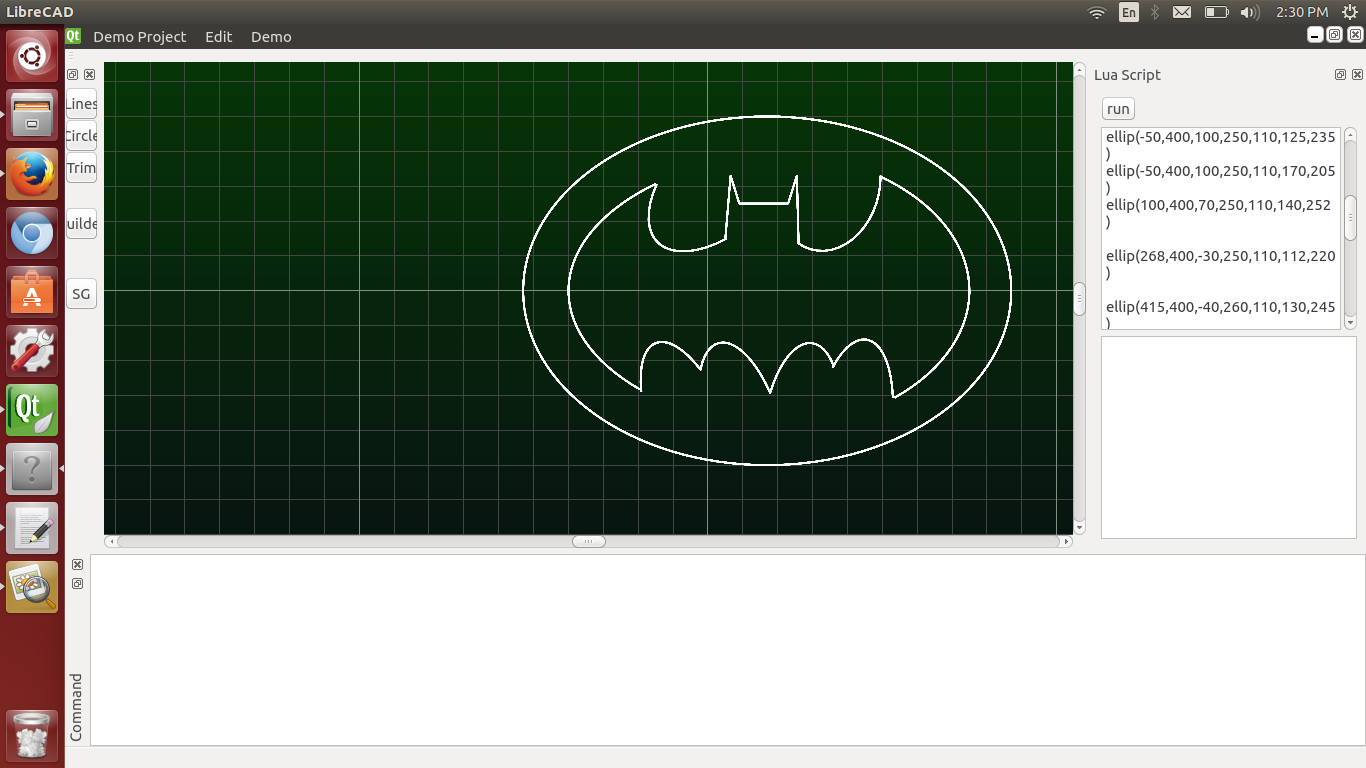
\includegraphics[scale=0.1]{batman.png}
\hspace*{1\baselineskip}
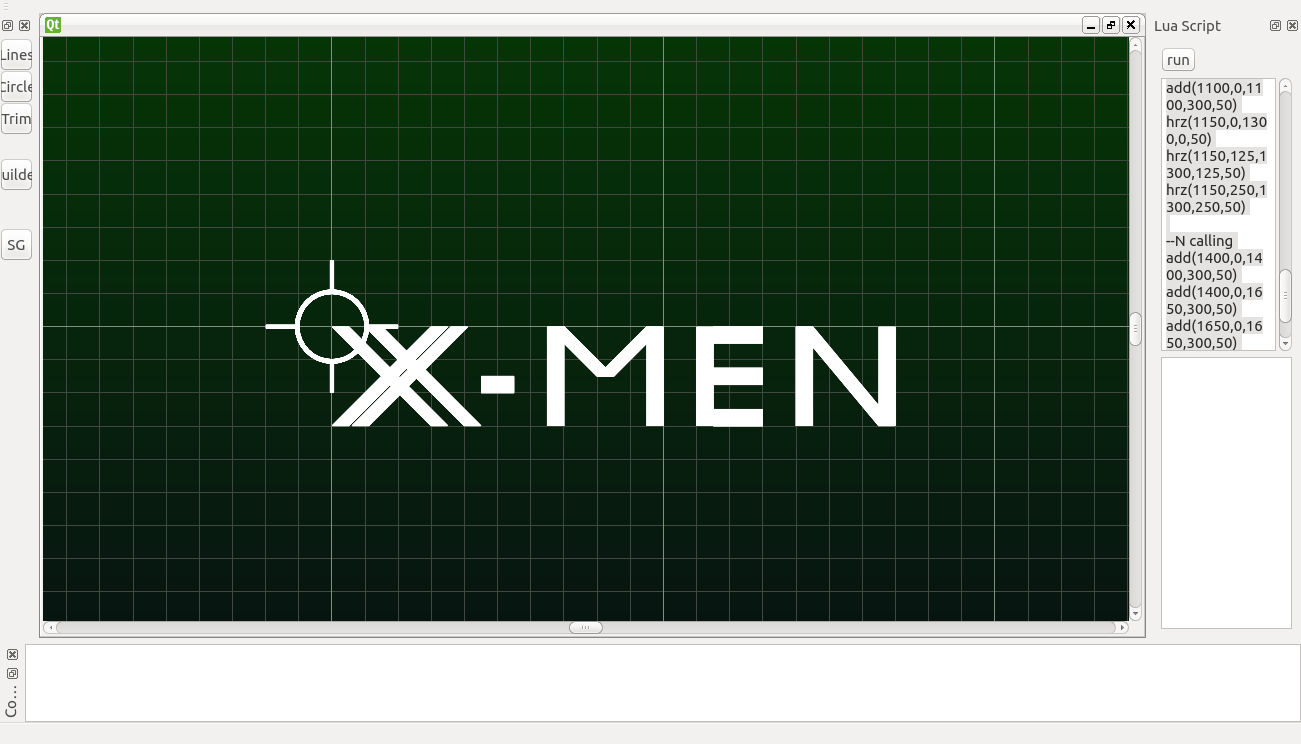
\includegraphics[scale=0.1]{xmenfinal.png}
\vspace*{1\baselineskip}
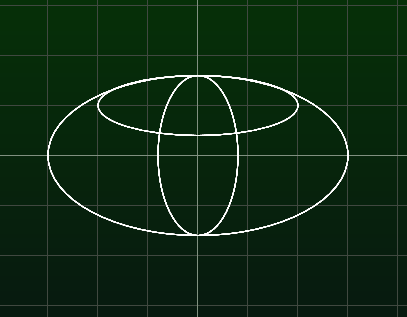
\includegraphics[scale=0.1]{toyota.png}
\hspace*{1\baselineskip}
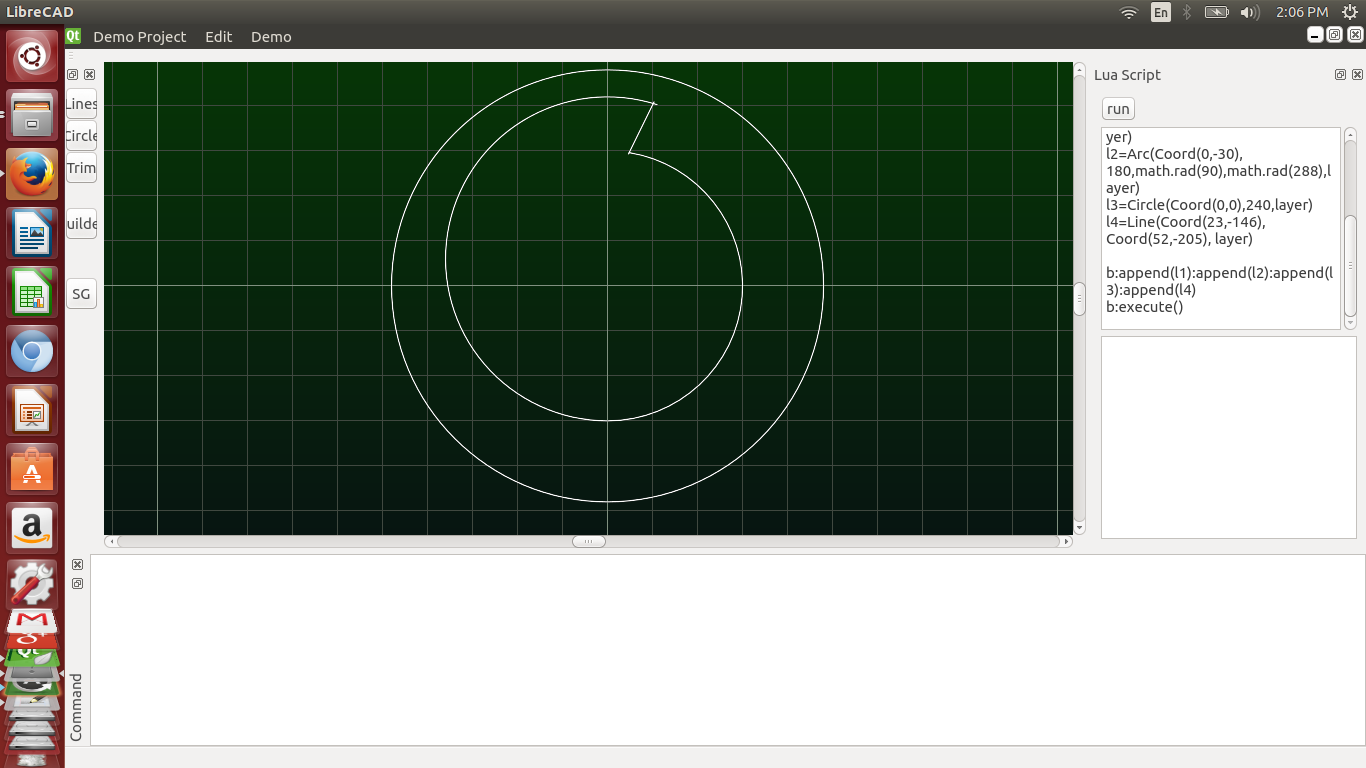
\includegraphics[scale=0.1]{vodafone.png}

\end{itemize}
\end{frame}

\begin{frame}[t,fragile]{Some Designs Using LUA in LibreCAD v3}

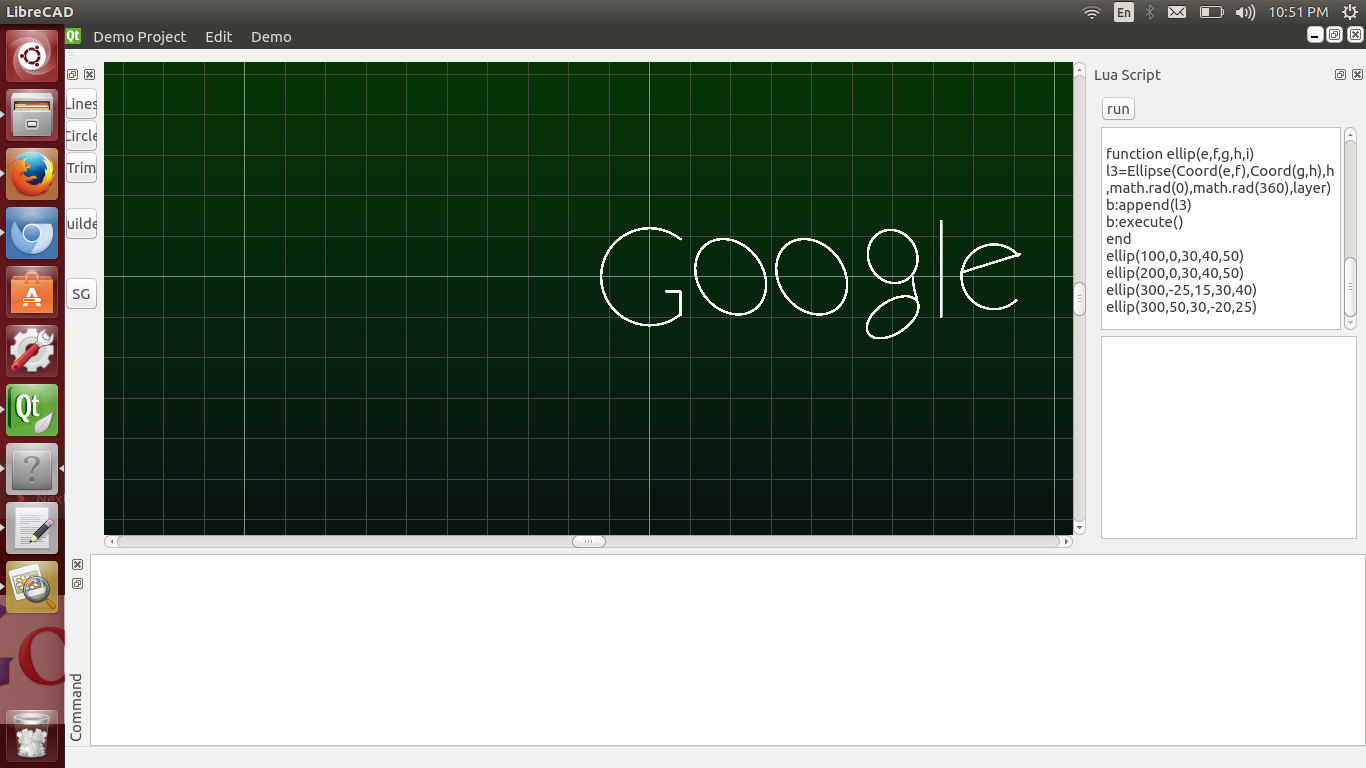
\includegraphics[scale=0.1]{google.png}
\hspace*{1\baselineskip}
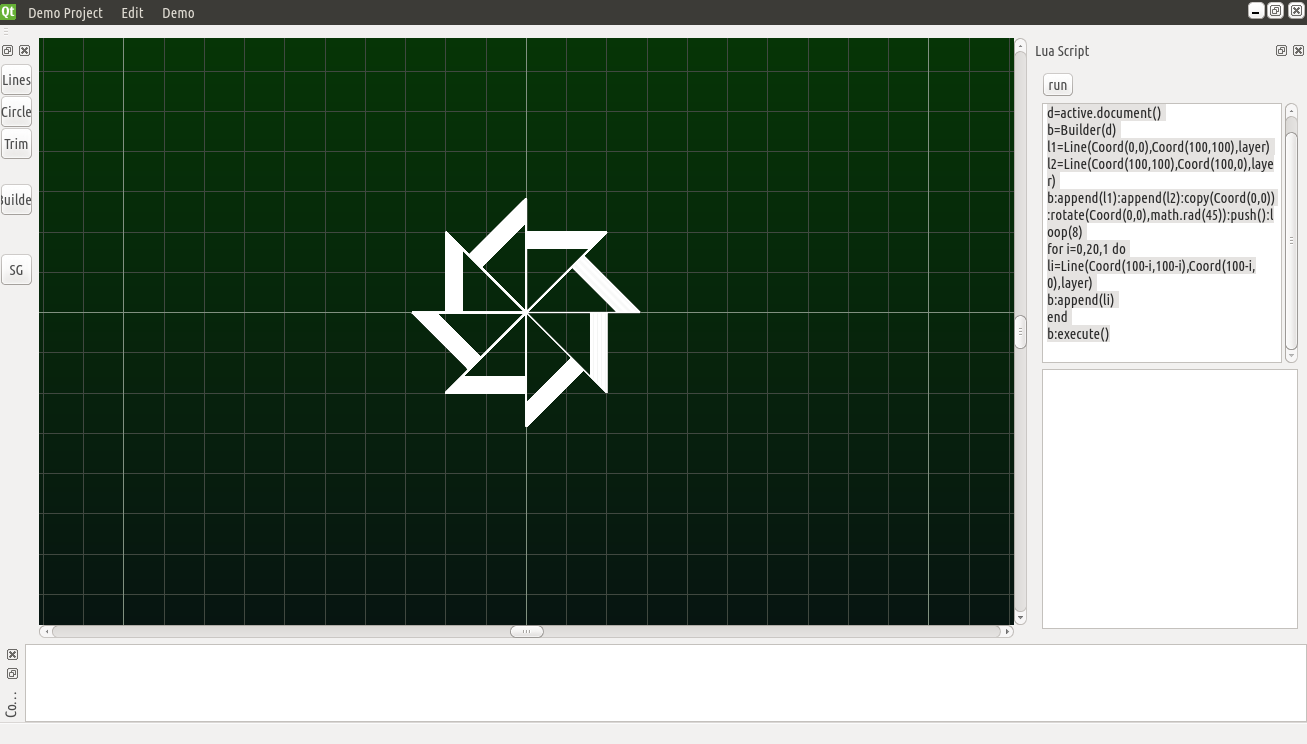
\includegraphics[scale=0.1]{chakra1.png}
\vspace*{1\baselineskip}
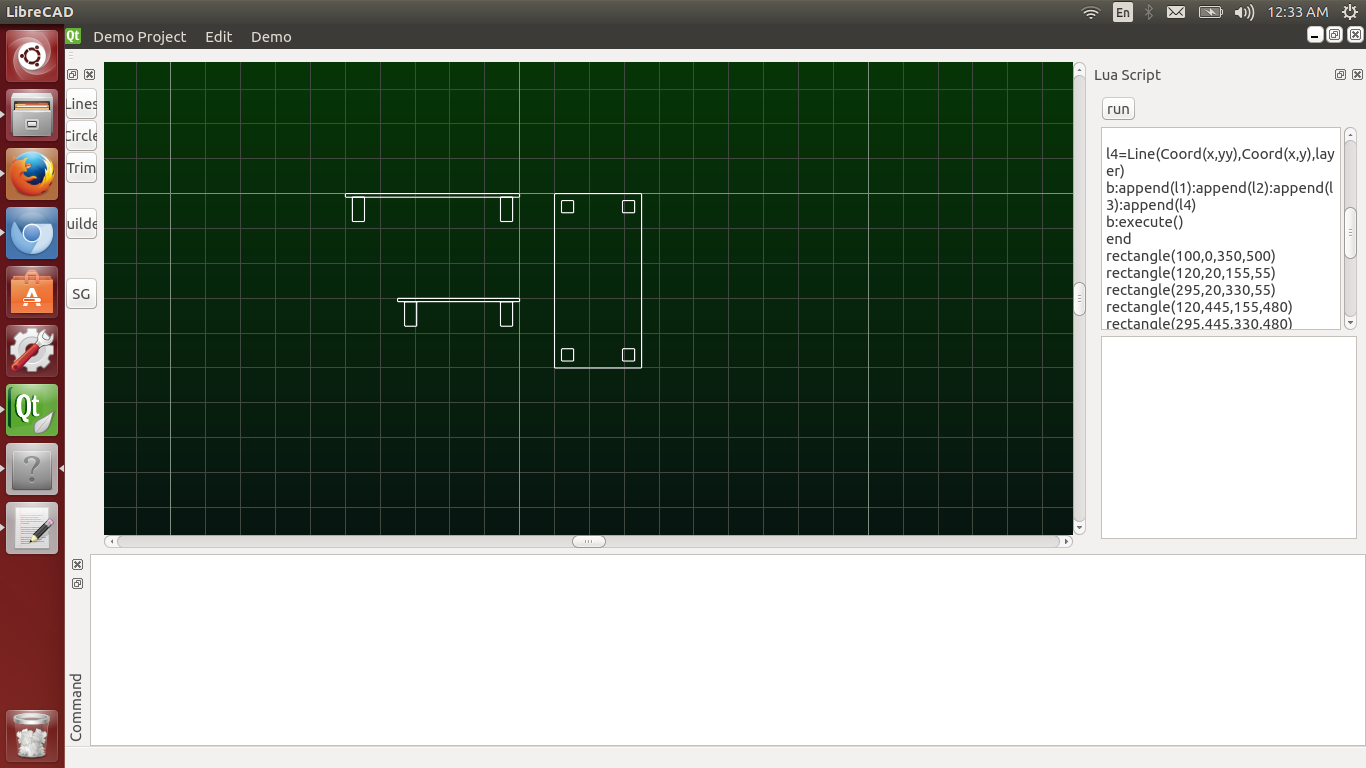
\includegraphics[scale=0.1]{table.png}
\hspace*{1\baselineskip}
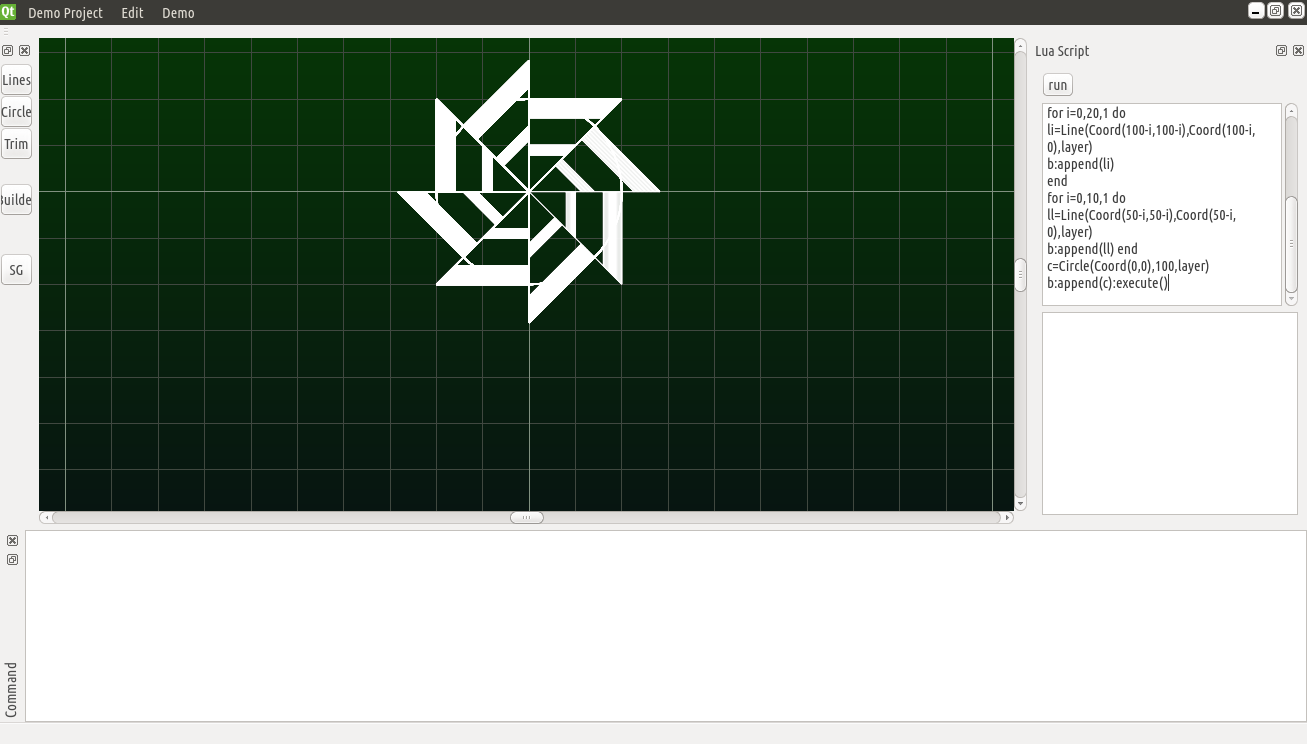
\includegraphics[scale=0.1]{chakra4.png}
\end{frame}

\begin{frame}[t,fragile]{Some Designs Using LUA in LibreCAD v3}
\begin{itemize}\item Water Tank\\

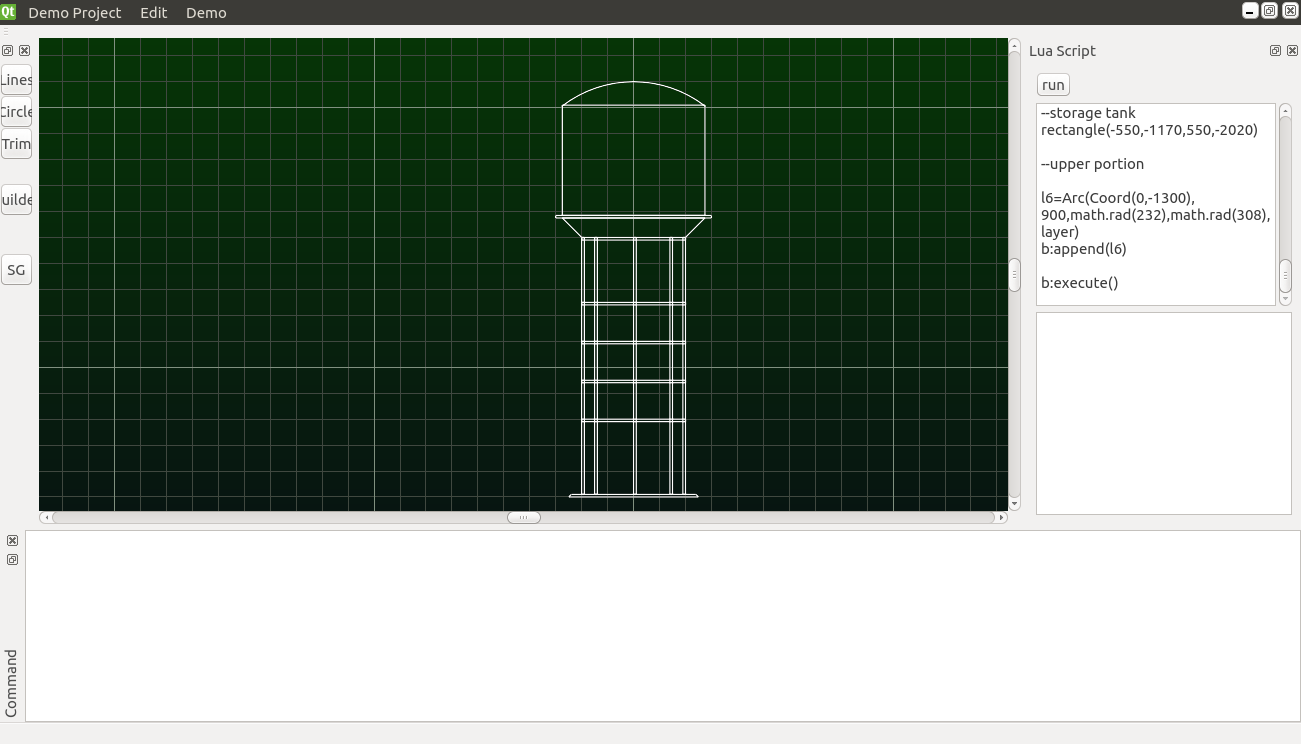
\includegraphics[scale=0.15]{tankside.png}
\hspace*{1\baselineskip}
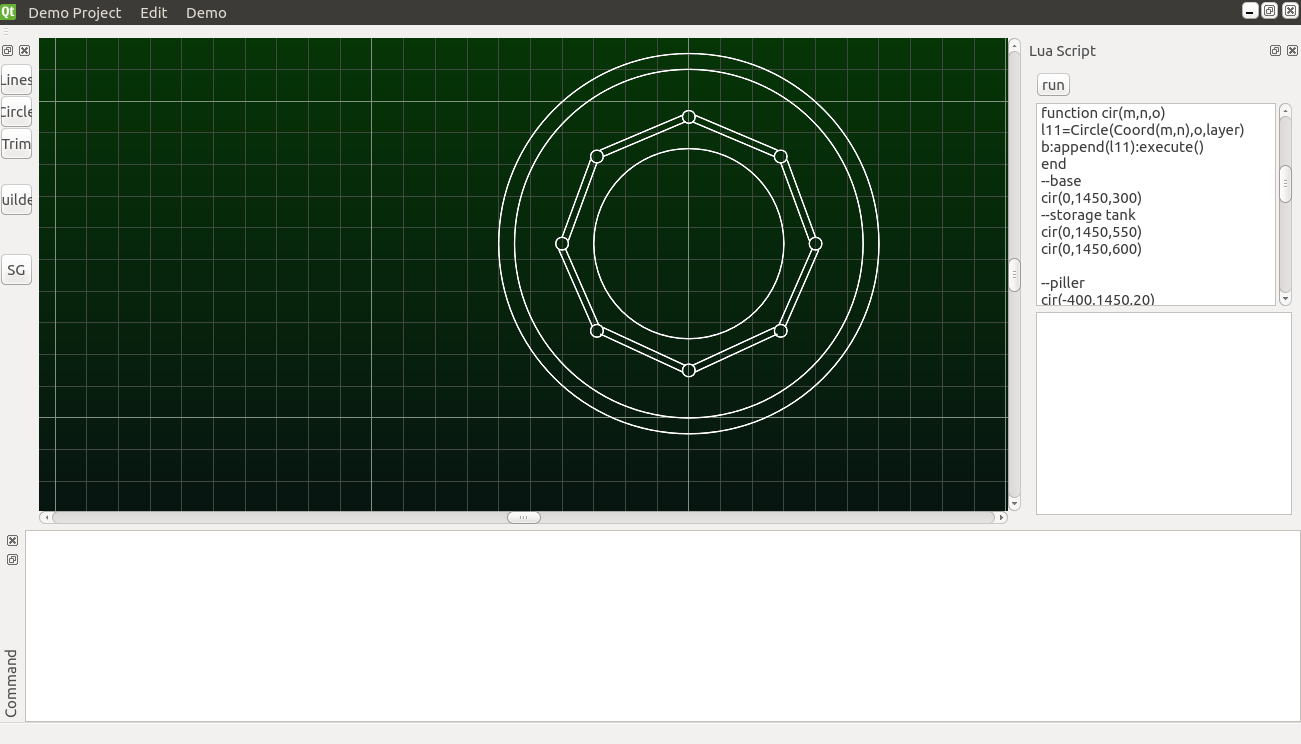
\includegraphics[height=90px,width=150px]{tanktop.png}
\end{itemize}
\end{frame}

\begin{frame}[t,fragile]{LibreOffice Draw UI Task}
\begin{itemize}
\item<1-> Our next task was to study the User Interface of LibreOffice Draw and to find some of its useful features and drawbacks.
\begin{itemize}\item<2-> After completion of this task we also give presentation on the advantages and limitations of LibreOffice Draw.
\end{itemize}
\item<3-> LibreOffice Draw is an excellent package for producing technical drawings, general posters etc.
\item<4-> Draw lets you manipulate graphical objects, group them, crop them, use objects in 3D and much more.

\end{itemize}
\end{frame}


\begin{frame}[t,fragile]{Hatching}
\begin{itemize}
\item<1-> We got another task to study about Hatching.
\item<2-> Hatching is a technique to fill a closed object with different patterns. 
\item<3-> Using cairo library we made simple program to fill a closed object with diferent patterns.
  \end{itemize}
\end{frame}
\watermarkon

\begin{frame}[t,fragile]{Other Learnings}
\begin{itemize}
\item<1-> Daily Dairy
\item<2-> Github
\item<3-> IRC
\item<4-> Vim
\item<5-> \LaTeX
\item<6-> Team Work
\end{itemize}
\end{frame}

\begin{frame}[t,fragile]{The End}
 THANK YOU !
\end{frame}

